\section*{TEMPLATE}
Le syllabus peut être trouvé à l'adresse \url{https://github.com/petervanroy/lingi1101}.
C'est de là que proviennent la majorité des templates utilisés dans ce solutionnaire, inspirez-vous en.\\
Lorsque vous trouvez une nouvelle structure qui n'a pas encore été employée dans ce rapport, tapez-en un exemple ici dans une section, en plus de la mettre dans votre partie.
(Et faites en sorte que ça compile!)
Comme ça les prochains pourront également s'en servir sans devoir fouiller partout.\\
Cette partie ne sera pas inclue dans le rapport final, elle sert uniquement lors de sa rédaction.

\subsection*{Quantificateurs et symboles}
\begin{itemize}
    \item \textbf{Et logique} : $\land$
    \item \textbf{Ou logique} : $\lor$
    \item \textbf{Négation} : $\neg$
    \item \textbf{Pour tout} : $\forall$
    \item \textbf{Il existe} : $\exists$
    \item \textbf{Implication} : $\Rightarrow$
    \item \textbf{Si et seulement si} : $\Leftrightarrow$
    \item \textbf{Tautologie} : $\models$
    \item \textbf{Conséquence logique} : $\Rrightarrow$
    \item \textbf{Équivalence logique} : $\Lleftarrow \Rrightarrow$
\end{itemize}


\subsection*{Règle - cas - résultat}
\begin{enumerate}
  \item Règle: $\forall$ $x$, $sac(x)$ $\Rightarrow$ $blanc(x)$
  \item Cas: $sac(a)$, $sac(b)$, $\cdots$\\
  \rule{5.5cm}{.1pt} 
  \item Résultat: $blanc(a)$, $blanc(b)$, $\cdots$
\end{enumerate}

\subsection*{Table de vérité}
\begin{center}
	\begin{tabular}{cc|ccccc}
		$P$ & $Q$ & $\lnot P$ & $\lnot Q$ & $\lnot( P \land Q)$ & $P \land Q$ & $ (\lnot P \lor \lnot Q)$\\
		\hline
		F&F&T&T&T&F&T\\
		T&F&F&T&T&F&T\\
		F&T&T&F&T&F&T\\
		T&T&F&F&F&T&F\\
	\end{tabular}
\end{center}

\subsection*{Règle BNF}
\begin{tabular}{rrl}
  $\textrm{<identificateur>}$ & ::= & $A$ | $B$ | $C$ | $D$ | \dots \\
  $\textrm{<proposition>}$
  & ::= & $\true$ \\
  & | & $\false$ \\
  & | & $\textrm{<identificateur>}$ \\
  & | & $(\textrm{<proposition>})$ \\
  & | & $\lnot \textrm{<proposition>}$ \\
  & | & $\textrm{<proposition>} \land \textrm{<proposition>}$ \\
  & | & $\textrm{<proposition>} \lor \textrm{<proposition>}$ \\
  & | & $\textrm{<proposition>} \Rightarrow \textrm{<proposition>}$ \\
  & | & $\textrm{<proposition>} \Leftrightarrow \textrm{<proposition>}$
\end{tabular}

%\subsection*{Pseudocode}

%\begin{algorithm}[H]
%\While{$false \not\in S$ et $\exists$? clauses résolvables non résolues}{
%	\begin{itemize}
%		\item choisir $C_1,C_2 \in S$ tel que $\exists P \in C_1, \lnot P \in C_2$ 		
%		\item calculer r:=$C_1 - \{P\} \lor C_2 - \{\lnot P\}$
%		\item calculer S:= $S \cup \{r\}$
%	\end{itemize}
%}
%\eIf{$false \in S$}{C est prouvé}{C n'est pas prouvé}
%\end{algorithm}

\subsubsection*{Exemple de résolution}
\begin{tabbing}
\hspace{3cm}\=\hspace{2cm}\=\kill
C$_{1}$ : P $\lor$ Q \\
C$_{2}$ : P $\lor$ R \\
C$_{3}$ : $\lnot$Q $\lor$ $\lnot$R \\
C : P \> \> \{C$_{1}$,C$_{2}$,C$_{3}$,$\lnot$C\}
\end{tabbing}

\noindent \emph{Quelques pas de résolution :}

\noindent C$_{1}$ + $\lnot$C $\rightarrow$  Q (C$_{5}$) \newline
C$_{2}$ + $\lnot$C $\rightarrow$ R  (C$_{6}$) \newline
C$_{3}$ + C$_{5}$ $\rightarrow$ $\lnot$R (C$_{7}$) \newline 
C$_{6}$ + C$_{7}$ $\rightarrow$ \underline{false} ($\in$ S donc C est prouvé) \newline


\subsubsection*{Preuve}

\begin{tabular}{|l|l|}
\hline
1. A$\Rightarrow$B & prémisse \\
2. C$\Rightarrow$D & prémisse \\
3. B$\lor$D $\Rightarrow$E & prémisse \\
4. $\lnot$E & prémisse \\ 
\indent 5. A & hypothèse \\
\indent 6. B & modus ponens (1) \\
\indent 7. B$\lor$D & addition (6) \\
\indent 8. E & modus ponens (7) \\
9. $\lnot$A & preuve indirecte \\
\indent 10. C & hypothèse \\
\indent 11. D & modus ponens (2) \\
\indent 12. D$\lor$B & addition (11) \\
\indent 13. B$\lor$D & commutativité (12)\\
\indent 14. E & modus ponens (9) \\
15. $\lnot$C & preuve indirecte \\
16. $\lnot$A $\land$ $\lnot$C & conjonction (9,15) \\
\hline
\end{tabular}\\

\subsection*{Tracer des graphes avec Tikz}

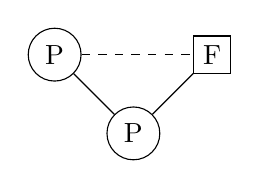
\begin{tikzpicture}
\coordinate (A) at (0,1);
\coordinate (B) at (1,0);
\coordinate (C) at (2,1);


\node[draw,circle] (A) at (A){P};
\node[draw,circle] (B) at (B){P};
\node[draw] (C) at (C){F};

\draw  (A)--(B);
\draw [dashed] (A)--(C);
\draw (C)--(B);

\end{tikzpicture}


